\documentclass{article}
\usepackage[spanish]{babel}
\usepackage[onehalfspacing]{setspace}
\usepackage[utf8]{inputenc}
\usepackage{amsmath}
\usepackage{amssymb}
\usepackage{verbatim}
\usepackage{graphicx}
\usepackage{listings}
\usepackage{fullpage}
\usepackage{color}
\usepackage{fancyvrb}
\usepackage{hyperref}
\hypersetup{%
	pdfborder = {0 0 0}
}

\definecolor{mygreen}{rgb}{0,0.6,0}
\definecolor{mygray}{rgb}{0.5,0.5,0.5}
\definecolor{mymauve}{rgb}{0.58,0,0.82}

\lstset{ %
	backgroundcolor=\color{white},   % choose the background color; you must add \usepackage{color} or \usepackage{xcolor}
	basicstyle=\footnotesize,        % the size of the fonts that are used for the code
	breakatwhitespace=false,         % sets if automatic breaks should only happen at whitespace
	breaklines=true,                 % sets automatic line breaking
	captionpos=b,                    % sets the caption-position to bottom
	commentstyle=\color{mygreen},    % comment style
	frame=single,                    % adds a frame around the code
	keepspaces=true,                 % keeps spaces in text, useful for keeping indentation of code (possibly needs columns=flexible)
	numbers=left,                    % where to put the line-numbers; possible values are (none, left, right)
	numbersep=5pt,                   % how far the line-numbers are from the code
	numberstyle=\tiny\color{mygray}, % the style that is used for the line-numbers
	rulecolor=\color{black},         % if not set, the frame-color may be changed on line-breaks within not-black text (e.g. comments (green here))
	showspaces=false,                % show spaces everywhere adding particular underscores; it overrides 'showstringspaces'
	showstringspaces=false,          % underline spaces within strings only
	showtabs=false,                  % show tabs within strings adding particular underscores
	stepnumber=1,                    % the step between two line-numbers. If it's 1, each line will be numbered
	stringstyle=\color{mymauve},     % string literal style
	tabsize=4,
	title=\lstname                   % show the filename of files included with \lstinputlisting; also try caption instead of title
}


\author{José Luis Cánovas Sánchez}
\title{ARQUITECTURAS DE REDES AVANZADAS\\QUAGGA}

\begin{document}
\maketitle

\begin{center}
	
\includegraphics[scale=0.3]{images/mascota.png}
\end{center}

\begin{abstract}
	En este informe se redacta el despliegue de un escenario de red IPv6 usando la herramienta Quagga.
\end{abstract}

\tableofcontents

\section{Introducción}

Quagga es un proyecto de software que provee de utilidades para encaminamiento de red en sistemas UNIX, con el demonio zebra permite aplicar las tablas de algoritmos de encaminamiento a las tablas de red de la máquina. Los algoritmos se ejecutan como demonios que toman la información de la red y aplican protocolos conocidos, tales como OSPF, RIP, IS-IS y BGP, en múltiples de sus versiones, y por medio de zebra los aplican a las tablas de red del sistema operativo.

\begin{center}
	\begin{BVerbatim}
+----+  +----+  +-----+  +-----+
|bgpd|  |ripd|  |ospfd|  |zebra|
+----+  +----+  +-----+  +-----+
|
+---------------------------|--+
|                           v  |
|  UNIX Kernel  routing table  |
|                              |
+------------------------------+

    Quagga System Architecture
	\end{BVerbatim}
\end{center}

Vamos a configurar un par de estos protocolos con Quagga en cuatro máquinas que harán las veces de routers.
En la sección 2 se muestra la topología que se va a implementar. En las secciones 3 a 6 se explicará cómo instalar y configurar Quagga con los mecanismos OSPFv3 y RIPng para IPv6.

La topología usada en este estudio de Quagga se asemeja mucho a la de la práctica 1 de ARA, pero se puede llevar a otros proyectos, como LEGO, fácilmente. Más adelante se muestra la topología en \autoref{fig:topology}, y con hacer corresponder R1 y R2 con los routers de las organizaciones de LEGO, las redes XXXX:\textbf{0:1}::/64 con las subredes de cada organización, y las subredes XXXX::/64 con una subred un nivel más interna, tenemos la topología de LEGO ampliada. La salida a internet se debería realizar con tunelado a IPv4 en R1 y R2, si no se dispone de IPv6 pública. En caso de tener un rango de direcciones IPv6 públicas, habría que cambiar los valores de cada subred para que sean válidos, pero queda fuera de este estudio.

\section{Topología de trabajo}


Partimos de dos Sistemas Autónomos con números 17 y 71 (curiosidad, son primos \hyperref{https://en.wikipedia.org/wiki/Permutable_prime}{}{}{\underline{permutables}}  entre sí) y mecanismo de encaminamiento interno por OSPF, con un área backbone y un área 1 stub para el AS17, un mecanismo basado en RIPng para el AS71 y rutas estáticas entre ambos AS, como se muestra en la \autoref{fig:topology}.


\begin{figure}[!h]
	\centering
	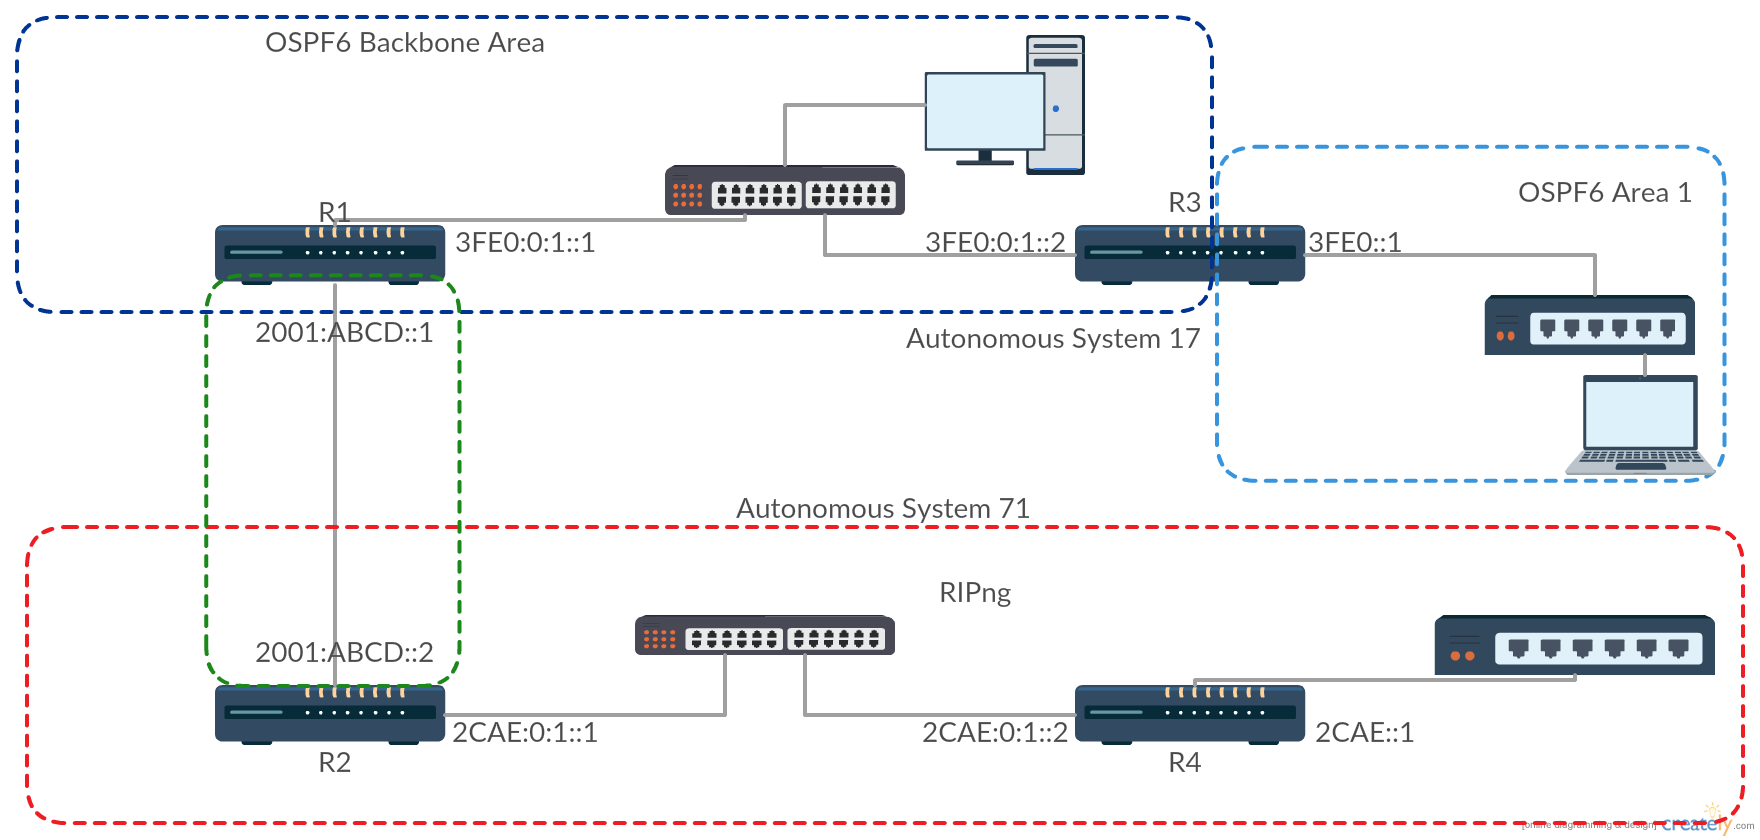
\includegraphics[scale=0.29]{images/Topology.png}
	\caption{Topología}
	\label{fig:topology}
\end{figure}

\hfill

Esta topología lógica la llevamos a la práctica con Virtual Box, con cuatro máquinas Debian sin interfaz gŕafica, y con tarjetas de red virtuales configuradas como redes internas del siguiente modo:

\begin{itemize}

	\item R1: Adaptador 1 Red Interna \textit{AS17} - Adaptador 2 Red Interna \textit{interAS}

	\item R2: Adaptador 1 Red Interna \textit{AS71} - Adaptador 2 Red Interna \textit{interAS}

	\item R3: Adaptador 1 Red Interna \textit{AS17} - Adaptador 2 Red Interna \textit{AS17Area1}

	\item R4: Adaptador 1 Red Interna \textit{AS71} - Adaptador 2 Red Interna \textit{AS71Subred}

\end{itemize}


\section{Instalar Quagga}

Para facilitar las pruebas, hay preparado un fichero Makefile que recibe como parámetro el router a configurar (r1, r2, r3 o r4), y ejecuta un script \textit{install.sh} que instala por aptitude el paquete \textit{quagga}.
 Con esto no es suficiente para que quagga funcione, ni tampoco para poder iniciar su consola de configuración. Para ello se crean en \textit{/etc/quagga/}
 los ficheros \textit{zebra.conf}, \textit{ospf6d.conf}, \textit{ripngd.conf} y \textit{vtysh.conf} con usuario quagga y grupo quaggavty.

 A todos los ficheros menos a \textit{vtysh.conf} se les añade la línea \textit{password pwd} donde pwd será la contraseña para poder configurar el demonio por su propia terminal. El fichero \textit{vtysh.conf} configura la terminal vtysh, que permite controlar todos los demonios, al estilo de la terminal de un router Cisco, y para mayor comodidad, se escribe \textit{username root nopassword} para no necesitar iniciar sesión cada vez que la usemos.

 Con esto los demonios podrían iniciarse sin problemas, pero falta decirle a Quagga qué demonios iniciar. Para ello el fichero \textit{/etc/quagga/daemons} se reescribe con:

 \begin{verbatim}
	 zebra=yes
	 bgpd=no
	 ospfd=no
	 ospf6d=yes
	 ripd=no
	 ripngd=yes
	 isisd=no
	 babeld=no
 \end{verbatim}

 Cambiando \textit{yes} o \textit{no} según queramos activar o no cada demonio. El de zebra es obligatorio si queremos que se apliquen las tablas de rutas de los demonios al sistema real, pero si sólo se quiere ejecutar el protocolo sin afectar a la máquina, para pruebas por ejemplo, se puede desactivar.

 En cuanto a que la máquina se quiera usar como router, se debe activar el forwarding de paquetes ipv6 a nivel de sistema operativo. En nuestro caso usamos la orden \textit{sysctl -w net.ipv6.conf.all.forwarding=1}. Además, para evitar que el router se configure en base a los router advertisement de otros routers, hay que poner a cero del mismo modo las siguientes variables: \textit{net.ipv6.conf.all.autoconf}, \textit{net.ipv6.conf.all.accept\_ra}, \textit{net.ipv6.conf.all.accept\_redirects}, \textit{net.ipv6.conf.all.router\_solicitations}. Para facilitar su ejecución en cada reinicio, existe una regla en el Makefile llamada \textit{ipv6forward} que ejecuta los comandos. Si se quiere evitar ejecutarlo cada vez que se inicia la máquina, basta modificar cada entrada correspondiente de \textit{/etc/sysctl}.


 Finalmente habría que reiniciar Quagga con \textit{/etc/init.d/quagga restart}, y existe también en el Makefile una regla llamada \textit{restart} para facilitarlo.
 
\section{Configuración de interfaces}

La configuración de \textit{/etc/network/interfaces} sería, por ejemplo, para R1:

\begin{BVerbatim}
auto lo
iface lo inet loopback

auto eth0
iface eth0 inet6 static
address 3FE0:0:1::1
netmask 64

auto eth1
iface eth1 inet6 static
address 3FE0::1
netmask 64
\end{BVerbatim}

\hfill


Pero nosotros vamos a configurarlo desde Quagga usando las órdenes (abriendo la terminal con sudo vtysh):

\hfil

\begin{BVerbatim}
configure terminal
	interface eth0
		no shutdown
		ipv6 address 3FE0:0:1::1/64
		no ipv6 nd suppress-ra
		ipv6 nd prefix 3fe0:0:1::/64 300 250 router-address
\end{BVerbatim}

\hfil

Y sustituyendo eth0 y la dirección ipv6 por cada interfaz correspondiente y su dirección. Las líneas que incluyen \textit{nd} (neighbour discovery) se incluyen para enviar Router Advertisements (no suppress-ra) y definir la información del Prefix Information Option del router advertisement (nd prefix). Con esto la interfaz queda configurada y actúa como router.


En los ficheros que usa el Makefile de instalación se incluyen las interfaces ya configuradas en zebra.conf (fichero que configura lo relativo a interfaces y la red en general, independiente del protocolo de enrutamiento).

En ese mismo fichero también se encuentran las rutas estáticas que deben conocer R1 y R2 para conocer la red del otro AS. Una ruta estática se indica en el estado de \textit{configure terminal} con \textit{ipv6 route X:X::X:X/X  Y:Y::Y:Y}, donde la primera dirección indica una subred con prefijo, y la segunda el gateway. Hay que tener cuidado con la ayuda de la terminal, pues también indica que se puede poner una interfaz como gateway, pero quagga tomará esa información como que la interfaz está conectada a dicha subred directamente.

\hfil

El fichero de configuración \textit{zebra.conf} de R1, como ejemplo, es:

\begin{lstlisting}
!
! Zebra configuration saved from vty
!   2015/11/22 19:55:56
!
password manyhue
!
interface eth0
ipv6 address 3fe0:0:1::1/64
no ipv6 nd suppress-ra
ipv6 nd prefix 3fe0:0:1::/64 300 250 router-address
!
interface eth1
ipv6 address 2001:ABCD::1/64
no ipv6 nd suppress-ra
ipv6 nd prefix 2001:ABCD::/64 300 250 router-address
!
interface lo
!
ipv6 route 2cae::/42 2001:abcd::2
!
!
!
line vty
!
\end{lstlisting}


\section{Configuración de OSPF}

La configuración por comandos de OSPFv3 partiendo del punto de entrada de \textit{sudo vtysh} sería:

\hfil

\begin{BVerbatim}
configure terminal
	router ospf6
		router-id a.b.c.d
		interface ethx area e.f.g.h
		redistribute connected
		redistribute static
		end
write
\end{BVerbatim}

Donde a.b.c.d se sustituye por un ID para el router en forma de dirección ipv4. Para R1 elegimos 1.1.1.1 y para R3 2.2.2.2.

Las áreas se identifican también con direcciones tipo ipv4 sustituyendo el valor en e.f.g.h, y nótese que no es necesario ir a la configuración de la interfaz y activar ahí ospf, quagga lo hace automáticamente desde la configuración de ospf al indicar la interfaz, aquí sustituyendo ethx por la interfaz correspondiente. Para las áreas la 0.0.0.0 será la backbone, y la 0.0.0.1 la segunda área de R3.

Para anunciar las redes que no están incluidas en las áreas de OSPF, se debe indicar con redistribute, en el caso de R1, connected y static.

Para R3 la línea de \textit{interface} habrá que ejecutarla una vez por cada una de las dos interfaces y sus áreas, y no haría falta el redistribute pues todas sus redes están en el AS gestionado con OSPF.

\hfill

Los ficheros de configuración generados al final por Quagga son casi idénticos a los de Cisco, y podrían ser la lista de comandos a ejecutar, excepto que añaden la información de las interfaces que deben usar ospf.

\hfil

El fichero de configuración \textit{ospf6d.conf} de R3, como ejemplo, es:

\begin{lstlisting}
!
! Zebra configuration saved from vty
!   2015/11/17 18:45:32
!
password manyhue
!
debug ospf6 lsa unknown
!
interface eth0
ipv6 ospf6 network broadcast
!
interface eth1
ipv6 ospf6 network broadcast
!
router ospf6
router-id 2.2.2.2
interface eth0 area 0.0.0.0
interface eth1 area 0.0.0.1
!
line vty
!
\end{lstlisting}


\section{Configuración de RIPng}

La configuración por comandos de RIPng partiendo del punto de entrada de \textit{sudo vtysh} sería:

\hfil

\begin{BVerbatim}
configure terminal
	router ripng
		network ethx
		redistribute connected
		redistribute static
		exit
	exit
write
\end{BVerbatim}

La configuración de RIPng es aún más sencilla que OSPF, donde además Quagga nos facilita el definir las redes a distribuir inticando directamente la interfaz donde antes pone network ethx.

Para que R2 anuncie las rutas a redes que quedan fuera del AS administrado por RIPng, al igual que en OSPF, se debe añadir la orden redistribute, anunciando las redes directamente conectadas y las indicadas por rutas estáticas.

En R4 no hacen falta las líneas \textit{redistribute} y habría que poner la orden network ethx por cada una de las dos interfaces que tiene y quedan dentro del AS.

Los ficheros de configuración del demonio ripngd generados son también parecidos a los de Cisco y en este caso son los comandos ejecutados antes:


\hfil

El fichero de configuración \textit{ripngd.conf} de R2, como ejemplo, es:

\begin{lstlisting}
!
! Zebra configuration saved from vty
!   2015/11/17 20:15:56
!
password manyhue
!
router ripng
network eth0
redistribute connected
redistribute static
!
line vty
!
\end{lstlisting}




\begin{thebibliography}{99}
	\bibitem{quaggaDoc}
	Documentación HTML de Quagga.  \hyperref{http://www.nongnu.org/quagga/docs/docs-info.html}{}{}{\underline{Link}}
	
	\bibitem{tipsandtricks}
	Tips \& tricks de Quagga. 
	\hyperref{https://wiki.quagga.net/wiki/index.php/TipsNTricks}{}{}{\underline{Link}}
	
\end{thebibliography}



\end{document}

